\documentclass{standalone}
%
\usepackage{tikz}
\usetikzlibrary{backgrounds,
%	bending,
%	arrows.meta,
%	shapes.callouts
}
%
\usepackage{tkz-euclide}
\usetkzobj{all}
%
\usepackage{dsfont}
%
\usepackage{xcolor}
%
\definecolor{space}{HTML}{1F2C4E}
\definecolor{earth}{HTML}{0089FA}
\definecolor{earthn}{HTML}{0C5898}
\definecolor{land}{HTML}{309347}
\definecolor{moon}{HTML}{AFAFAF}
\definecolor{craterm}{HTML}{616060}
\definecolor{linem}{HTML}{DBDBDB}
%
\usepackage{amsmath}
%
\usepackage{fontspec}
\setmainfont{Open Dyslexic}
%
\title{Sistema Terra-Luna}
\begin{document}
	\tikzset{
		partial ellipse/.style args = {#1:#2:#3}{insert path={+ (#1:#3) arc (#1:#2:#3)}},
	}
	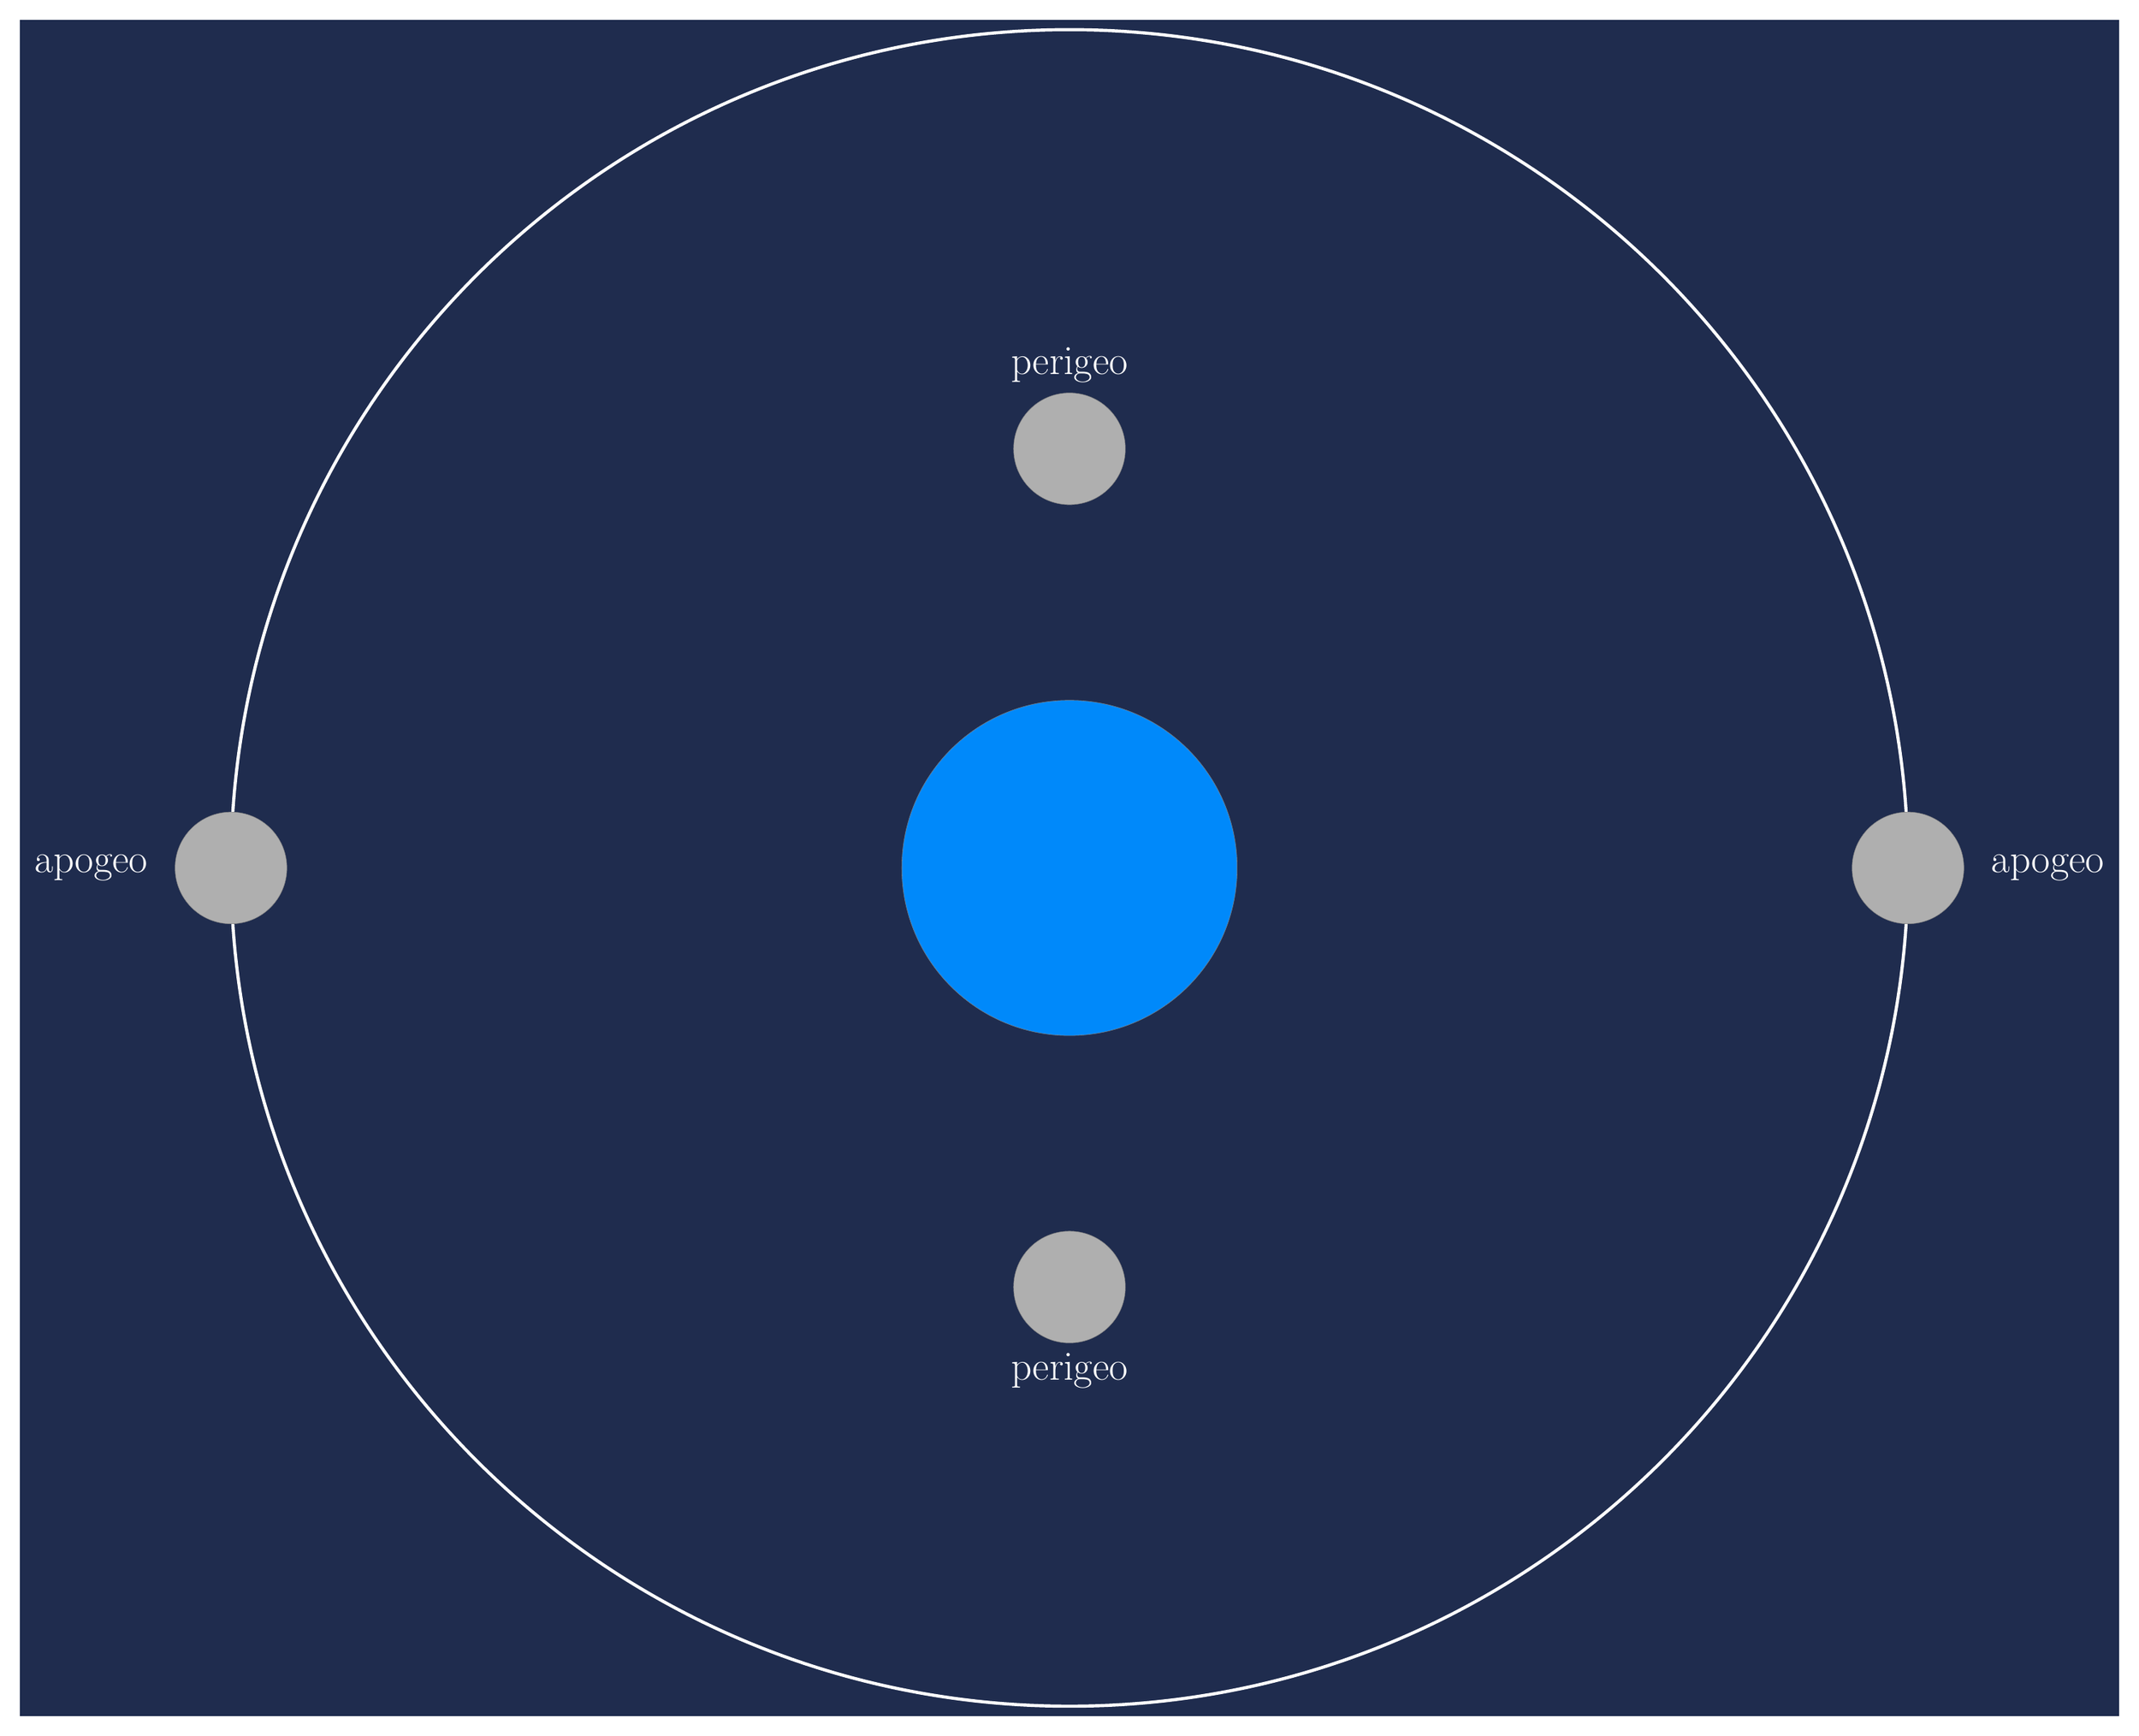
\begin{tikzpicture}[background rectangle/.style={fill=space},show background rectangle]
		\tkzDefPoint(0,0){E}
		\tkzDefPoint(3,0){Er}
		\tkzDefPoint(15,0){L}
		\tkzDefPoint(16,0){Lr}
		%
		\begin{scope}[yscale=0.5]
			\tkzDrawCircle[color=white,ultra thick](E,L)
		\end{scope}
		%
		\tkzDrawCircle[fill=earth](E,Er)
		\tkzDrawCircle[fill=moon](L,Lr)
		%
		\tkzDefPoint(0,7.5){L1}
		\tkzDefPoint(1,7.5){Lr1}
		\tkzDrawCircle[fill=moon](L1,Lr1)
		%
		\tkzDefPoint(-15,0){L2}
		\tkzDefPoint(-16,0){Lr2}
		\tkzDrawCircle[fill=moon](L2,Lr2)
		%
		\tkzDefPoint(0,-7.5){L3}
		\tkzDefPoint(1,-7.5){Lr3}
		\tkzDrawCircle[fill=moon](L3,Lr3)
		%
		\node at (17.5,0) {\textcolor{white}{\fontsize{20}{21}\selectfont apogeo}};
		\node at (-17.5,0) {\textcolor{white}{\fontsize{20}{21}\selectfont apogeo}};
		\node at (0,9) {\textcolor{white}{\fontsize{20}{21}\selectfont perigeo}};
		\node at (0,-9) {\textcolor{white}{\fontsize{20}{21}\selectfont perigeo}};
	\end{tikzpicture}
%
\end{document}